\section{Linux Desktop} 

  The following set of notes describes the everyday use of a Linux operating system. I refer to it for mainly my personal desktop, but it is also useful for working in computing clusters. Some of the commands are specific to the Arch Linux distribution (since that is what I work with), but I occasionally include those from Ubuntu and Red Hat, since I run into these distributions often in servers. 

  I try to organize this in a way so that one who wishes to get started in Linux can go through these notes chronologically. For now, we will assume that you have a Linux distribution installed. There are many resources beyond this book that helps you do that. 

  You can always try out Ubuntu (or any other distribution) through a \textbf{virtual machine}, which is a software emulation of a physical computer system. It allows you to run multiple operating systems or instances of an operating system on a single physical machine. Each virtual machine operates independently and has its own virtual hardware, including virtual CPU, memory, storage, and network interfaces. Virtual machines are created and managed by virtualization software called \textbf{hypervisors}. The hypervisor abstracts the underlying physical hardware and allows multiple virtual machines to share the same resources while isolating them from one another. This enables efficient utilization of hardware resources and provides flexibility in deploying and managing various operating systems and software applications. VMs generally have the advantage of being completely isolated from the main computer, so if anything wrong happens in the VM, it's fine. They can be used in research environments that are beta-testing unstable packages or for white-hacking practices. One example of a hypervisor is Oracle's \textbf{VirtualBox}, which is free to download. It should look like this when you open it for the first time. 
  \begin{center}
      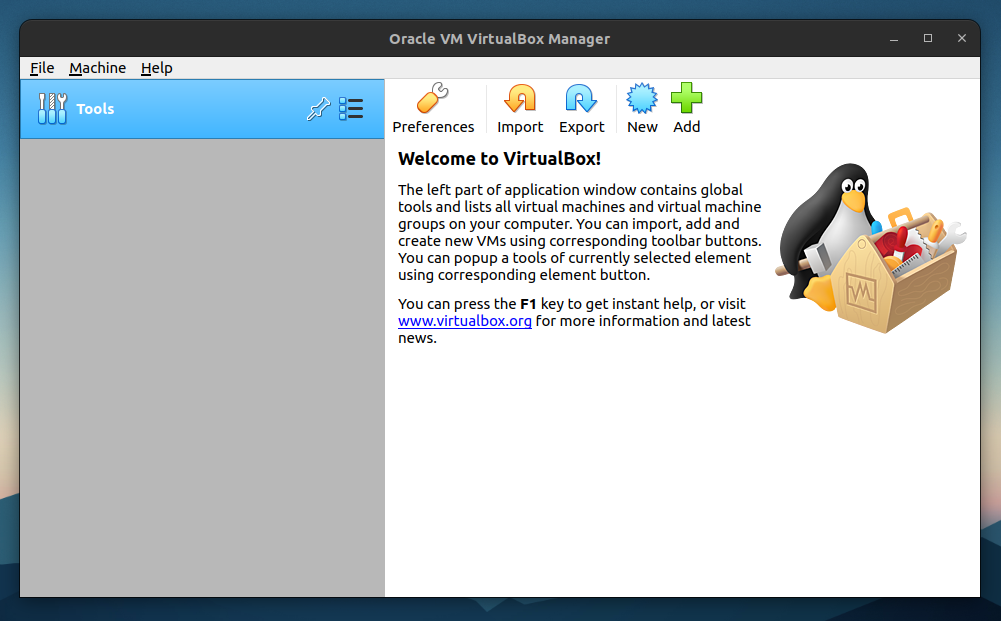
\includegraphics[scale=0.2]{img/VirtualBox.png}
  \end{center}
  Now in order to create a VM with its own OS, you need to have the appropriate \textbf{ISO file}, which is an exact copy of an entire optical disk such as a CD, DVD, or Blu-ray archived into a single file. The essentially stores the entire software needed to operate the OS. Therefore, you should download the proper ISO file from the internet (usually a couple GBs). 
  \begin{enumerate}
      \item \href{https://ubuntu.com/download/desktop}{Ubunutu ISO files}
      \item \href{https://www.microsoft.com/en-us/software-download/windows10}{Windows 10 ISO files}
      \item Apple does not allow distribution of its ISO files, so you will need to download from unofficial sources, which may be unsafe. 
  \end{enumerate}
  Once you have this ISO file, you can reuse it to create as many VMs as you want of that OS. Now follow these instructions: Click the new button and select where the virtual machine data will be stored, along with its OS. You can set the RAM, but don't make it more than half of your host computer since it will hog up too much RAM. Choose ``Create a virtual hard disk now". Choose ``VDI (VirtualBox Disk Image)". Dynamically allocated just means that the virtual disk size will adaptively grow as your storage gets full. Set the disk size to be at least 20GB. 

  After you created this, go to the VM settings (this is where you can edit your CPU cores, RAM cap, etc.). To add the ISO file, click on the ``Empty" tab right under the ``Controller:IDE", then the CD icon to the right, and ``choose a disk file". You should now choose the ISO file. Then go tweak other settings, and set the display:video memory to the max (128MB). Now you should be able to go through the installation wizard when you turn the VM on. 
  \begin{figure}[hbt!]
      \centering 
      \begin{subfigure}[b]{0.45\textwidth}
      \centering
          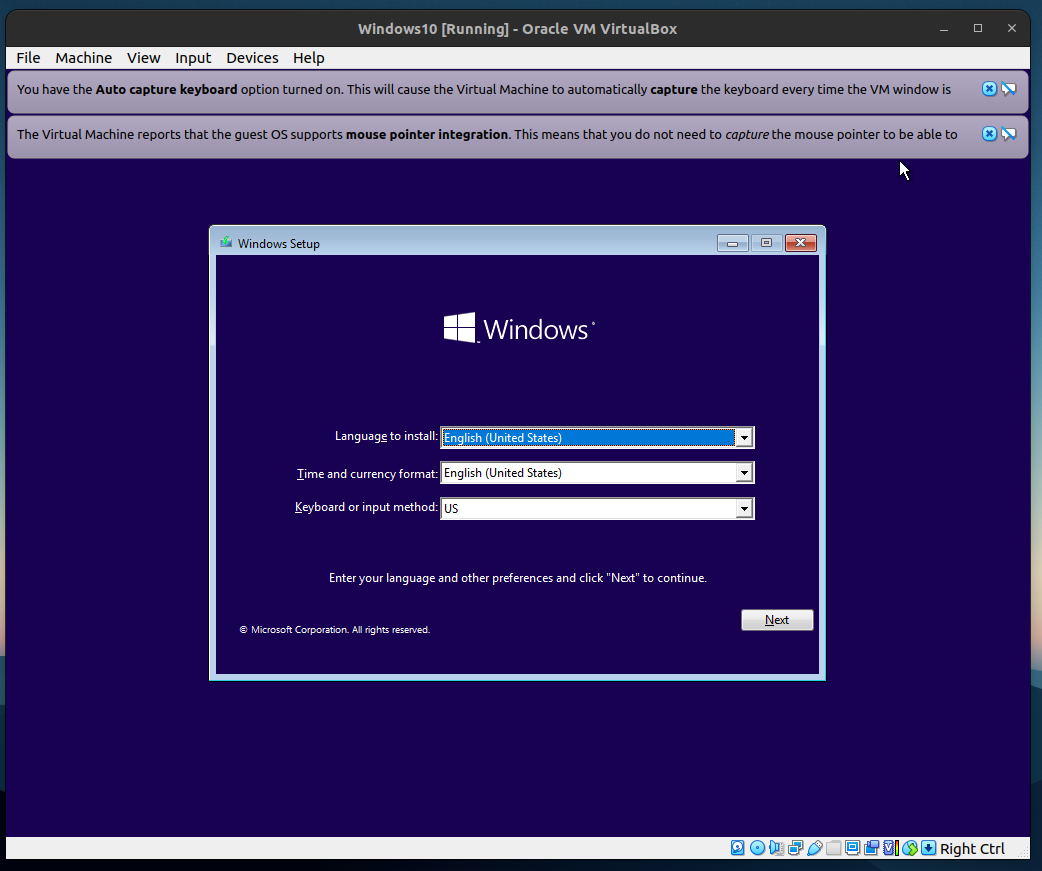
\includegraphics[width=\textwidth]{img/VM_Windows1.png}
          \caption{Windows 10 Set Up}
          \label{fig:VM_Windows1}
      \end{subfigure}
      \hfill 
      \begin{subfigure}[b]{0.45\textwidth}
      \centering
          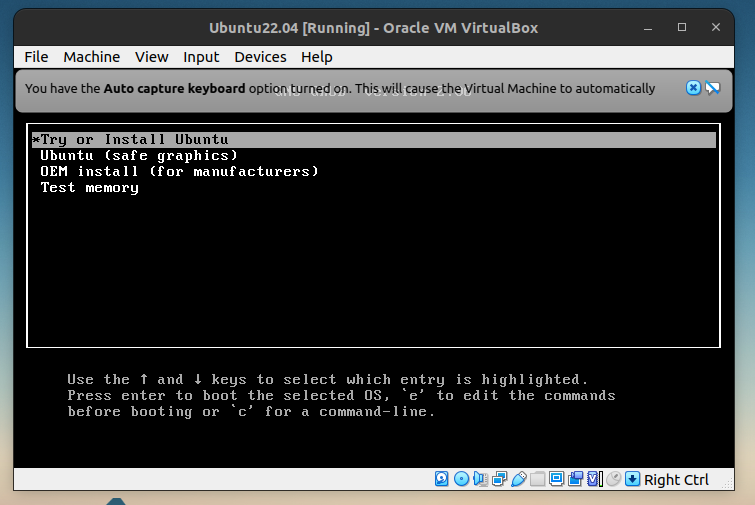
\includegraphics[width=\textwidth]{img/VM_Ubuntu1.png}
          \caption{Ubuntu 22.04 Set Up}
          \label{fig:VM_Ubuntu1}
      \end{subfigure}
      \caption{What you should get once you open up the VM after adding ISO files. }
  \end{figure}
  Refer to the instructions for each OS. 
  \begin{enumerate}
      \item For Windows: Say I don't have a product key. Click Windows 10 Home. Accept terms. Select the custom installation. Click the drive and click new, making the parititon at least 10534MB, and click apply. Next. Wait for the system to load. 
      \item For Ubuntu, you should get a GRUB view. Select ``Try or install Ubunutu". 
  \end{enumerate}
  You should now see one of these two screens. 
  \begin{figure}[hbt!]
      \centering 
      \begin{subfigure}[b]{0.45\textwidth}
      \centering
          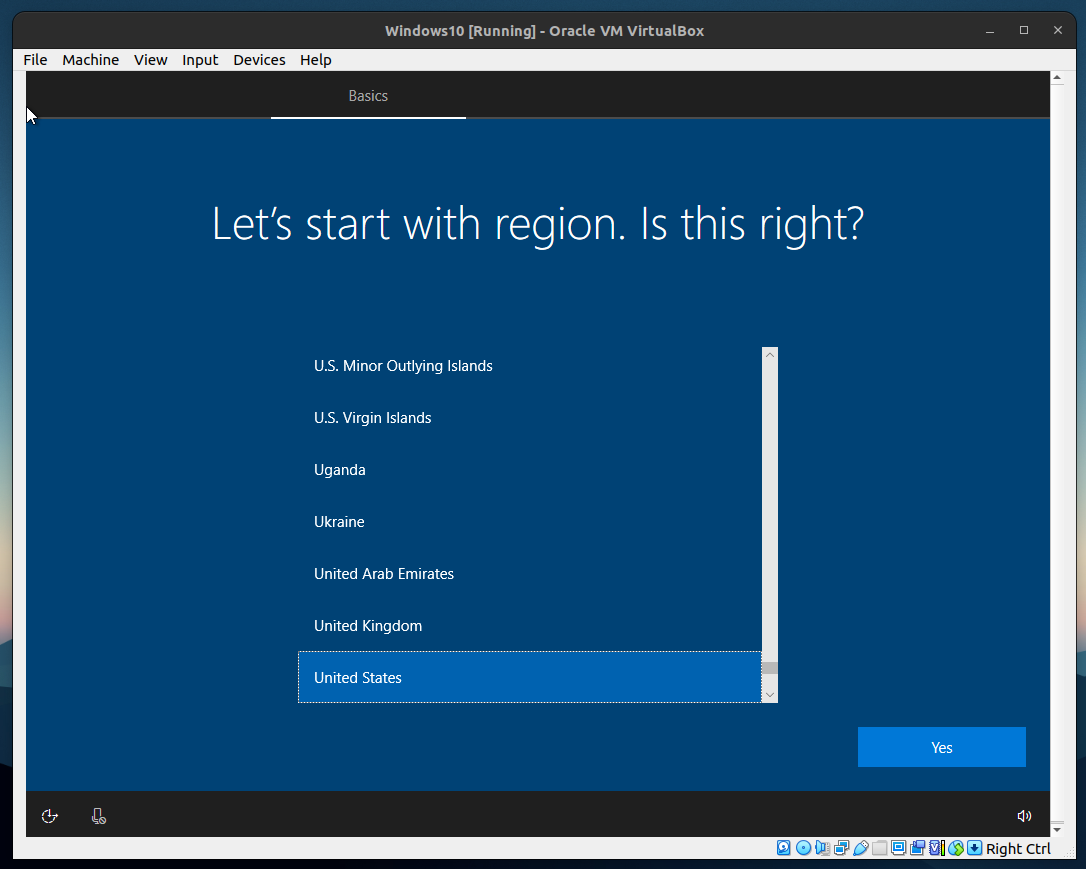
\includegraphics[width=\textwidth]{img/VM_Windows2.png}
          \caption{Windows 10 Set Up}
          \label{fig:VM_Windows2}
      \end{subfigure}
      \hfill 
      \begin{subfigure}[b]{0.45\textwidth}
      \centering
          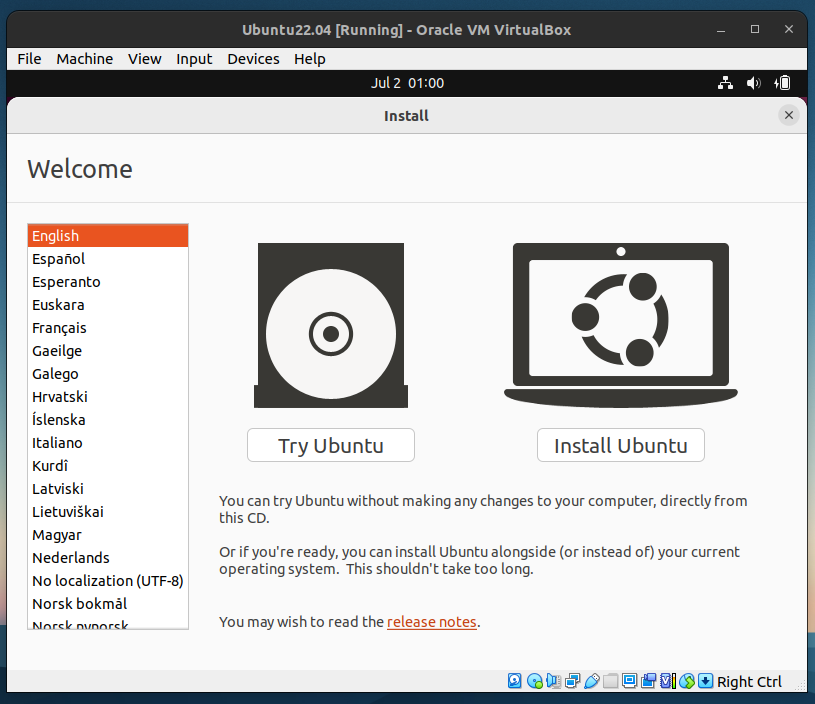
\includegraphics[width=\textwidth]{img/VM_Ubuntu2.png}
          \caption{Ubuntu 22.04 Set Up}
          \label{fig:VM_Ubuntu2}
      \end{subfigure}
      \caption{What you should get once you open up the VM after initial configuration and log in. }
  \end{figure}
  \begin{enumerate}
      \item For Windows, select your region. Select the keyboard layout. Sign in or create a Microsoft account. Choose privacy terms. Skip whatever. 
      \item For Ubuntu: Select Install Ubuntu with English. Set the keyboard layout. The normal installation may take a while, so I would select minimal depending on what you need. If you are short on time, you can uncheck the download updates while installing since you can always do that after you install. Click Erase disk and install Ubunutu. Choose region and add information. 
  \end{enumerate}
  Finally, you should see your desktop. 
  \begin{figure}[hbt!]
      \centering 
      \begin{subfigure}[b]{0.45\textwidth}
      \centering
          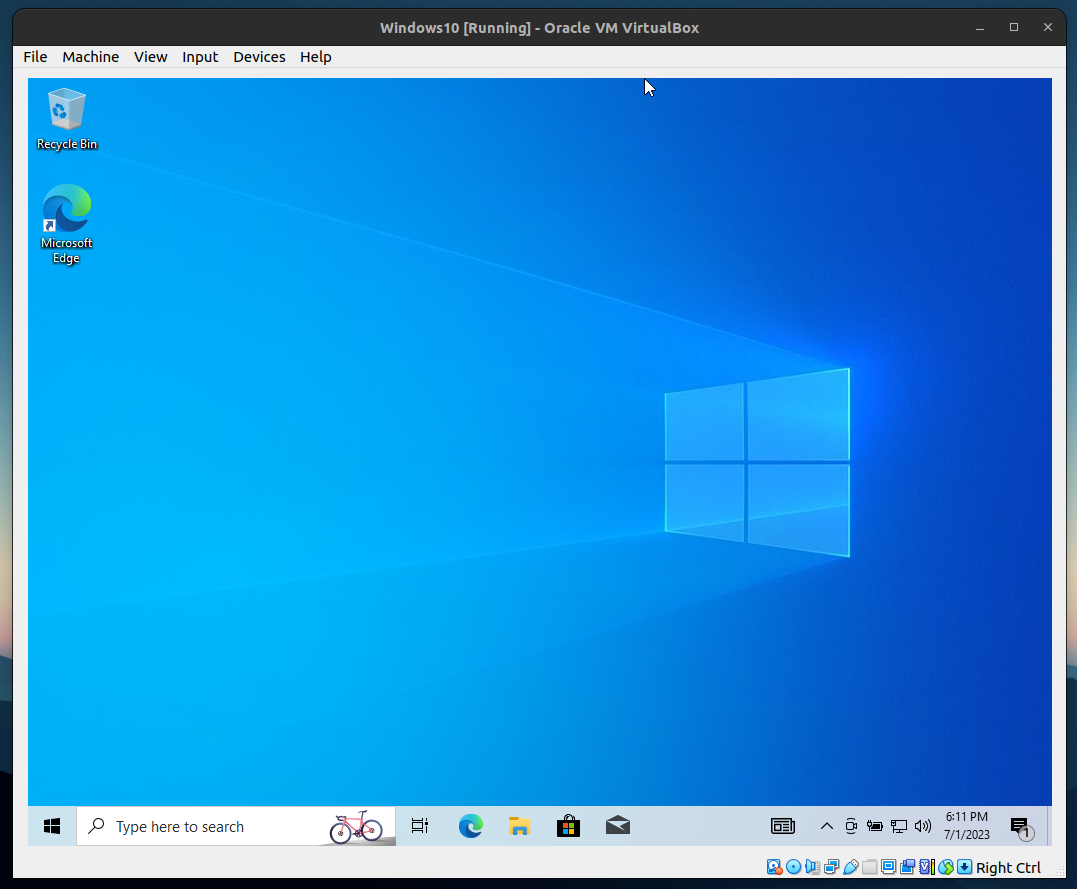
\includegraphics[width=\textwidth]{img/VM_Windows3.png}
          \caption{Windows 10 Set Up}
          \label{fig:VM_Windows3}
      \end{subfigure}
      \hfill 
      \begin{subfigure}[b]{0.45\textwidth}
      \centering
          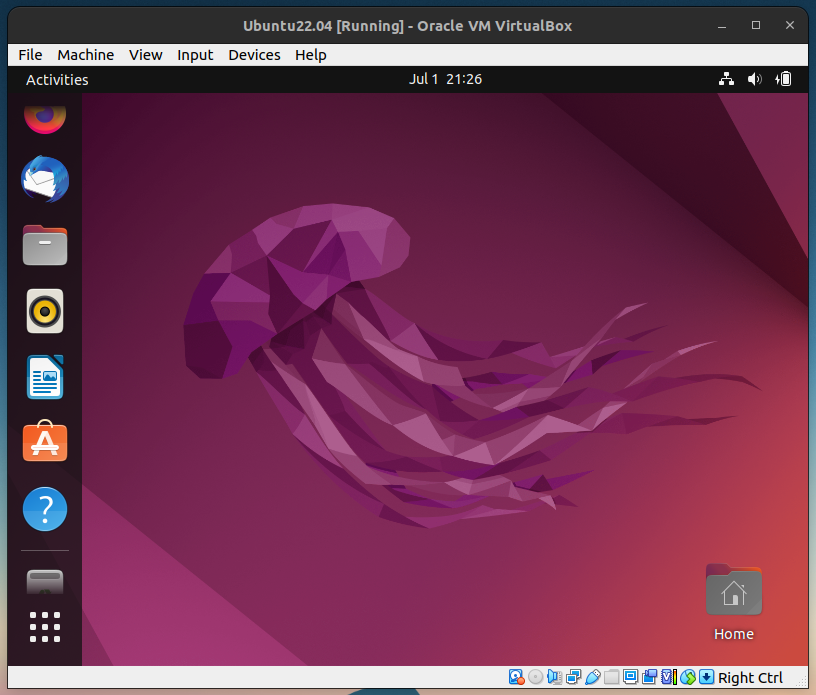
\includegraphics[width=\textwidth]{img/VM_Ubuntu3.png}
          \caption{Ubuntu 22.04 Set Up}
          \label{fig:VM_Ubuntu3}
      \end{subfigure}
      \caption{What you should see once everything is set up. }
  \end{figure}

  For my personal use, the packages below are ones that I end up installing every time I create a new VM to work in during research. 

  \begin{lstlisting}
    sudo apt update
    sudo apt install snapd
    sudo snap install --classic code
    sudo snap install slack
    sudo apt install git 
    sudo snap install spotify 
    sudo apt install htop
    wget https://dl.google.com/linux/direct/google-chrome-stable_current_amd64.deb
    sudo dpkg -i google-chrome-stable_current_amd64.deb
    sudo apt install virtualbox 
  \end{lstlisting}

  Once you are ready to use Linux consistently, it is optimal to \textbf{dual boot} it, which means that you have one computer that is divided into two: one for each operating system. Then you need to partition your drive and allocate it to your secondary OS. There are plenty of guides and tutorials online on how to do this. 

  There may be a point where you may need to resize your drive partitions as you need more or less space in one of your OS. This is when we need to do \textbf{partition resizing}. To do this, we need an empty thumb drive with at least 8GB of space in it (everything in here will be deleted). Then in your Ubuntu, install balenaEtcher and an Ubuntu (any version) ISO file. Mount the ISO file into your USB drive using balenaEtcher, following the steps in \href{https://www.youtube.com/watch?v=Kyz9x71gEPI&t=504s}{this video} to eventually get into Gparted. Another popular \href{https://www.youtube.com/watch?v=vlVXPtJ20hA&t=467s}{guide} uses Rufus in the Windows system, but I have found that this does not work for me. 

\subsection{Systemd} 

  A \textbf{process} is really any program that is running on your computer. A \textbf{daemon} is a background process that runs continuously, performing specific tasks even when no user is logged in. 

  Once the kernel has been loaded and completed its initialization process, it creates a collection of \textit{spontaneous} (as in the kernel starts them automatically) processes in user space. They're really part of the kernel implementation and don't necessarily correspond to programs in the filesystem. They're not configurable and they don't require administrative attention. These processes can be monitored with the commands \texttt{ps}, \texttt{top}, or \texttt{htop}.

  The most important process is the init process, with a system PID of 1 and with special privileges. It is used to get the system running and for starting other processes. 

  \begin{enumerate}
    \item Setting the name of the computer 
    \item Setting the time sone 
    \item Checking disks with \texttt{fsck} 
    \item Mounting filesystems 
    \item Removing old files from the \texttt{/tmp} directory 
    \item Configuring network interfaces
    \item Configuring packet filter 
    \item Starting up other daemons and network services, along with killing zombie processes or parenting orphaned processes. 
  \end{enumerate}

  There are three flavors of system management processes in widespread use: 
  \begin{enumerate}
    \item Historically, SysVinit was a series of plaintext files that ran as scripts to start processes, but due to some problems, Linux now uses systemd.
    \item An init variant that derives from the BSD UNIX, used on most BSD-based systems. 
    \item A more recent contender called \textbf{systemd} which aims to cover the init processes and much more. This significant increase in control causes some controversy. 
    \item Other flavors include Apple MacOS's \textbf{launchd} before it adopted systemd. Ubuntu also used \textbf{Upstart} before migrating to systemd. 
  \end{enumerate}

  Systemd is essentially a collection of smaller programs, services, and libraries such as systemctl, journalctl, init, process management, network management, login management, logs, etc. Some processes may depend on other processes, and with hundreds of them, it's very hard to do manually, which is why systemd does it all for you. A post on the systemd blog notes that a full build of the project generates 69 different binaries (subject to change). 

  \begin{definition}
    A \textbf{unit} is anything that is managed by systemd. It can be ``a service, a socket, a device, a mount point, an automount point, a swap file or partition, a startup carget, a watched filesystem path, a time controlled and supervised by systemd, a resource management slice, or a group of externally created processes." Within systemd, the behavior of each unit is defined and configured by a \textbf{unit file}. Within systemd, the behavior of each unit is defined and configured by a \textbf{unit file}. 

    The files are all over the place: 
      \begin{enumerate}
        \item \texttt{/lib/systemd/system} contains standard systemd unit files 
        \item \texttt{/usr/lib/systemd/system} are from locally installed packages, e.g. if I installed a pacman package that contained unit files, then those would go here. 
        \item \texttt{/etc/systemd/system} is where you put your custom files. etc also has the highest priority, so it overwrites the other files.  
        \item \texttt{/run/systemd/system} is a scratch area for transient units. 
      \end{enumerate}

    By convention, unit files are named with a suffix that varies according to the type of unit being configured. For example, service units have a \texttt{.service} suffix and timers user \texttt{.timer}. Within the unit file, some sections e.g. (\texttt{[Unit]}) apply generically to all kinds of units, but others (e.g. \texttt{[Service]}) can appear only in the context of a particular unit type. 

  \end{definition}

  \begin{example}[Service Unit File]
    If we go into one of these unit files, which have the prefix \texttt{.service}, they are usually formatted as such: 

    \begin{lstlisting}
      # comments are just the same as in bash Scripts
      # the headers are important! 

      [Unit]        #  
      Description=Description of the unit file 
      Documentation=man:something 
      After=network.target

      [Service]
      Type=forking  # tells that the process may exit and is not permanent
      PIDFile=      # 
      ExecStartPre= # scripts to run before you start 
      ExecStart=    # scripts to run when starting 
      ExecReload=   # script to run when you try to reload the process
      ExecStop=     # script to run to stop the process 

      [Install]   # Tells at what point should this be running
      WantedBy=multi-user.target 

    \end{lstlisting} 
  \end{example}
  
\subsubsection{systemctl: Managing systemd} 

  \textbf{systemctl} is an all-purpose command for investigating the status of systemd and making changes to its configuration. Running \texttt{systemctl} without any arguments invokes the default \texttt{list-units} subcommand, which shows all loaded and activive services, sockets, targets, mounts, and devices. To show only services, use \texttt{--type=service}. 

  The two main commands that you will use to interact with systemd is \texttt{systemctl} and \texttt{journalctl}. 
  
  \begin{enumerate}
    \item \texttt{systemctl status unit} checks the status, ouputting the description, whether it's enabled/disabled, and whether it's active/inactive. 
    \item \texttt{systemctl enable unit} enables it, which means that it will start when booting the computer. It does this by creating a symlink to the unit file. This is different from start. 
    \item \texttt{systemctl disable unit} disables it. 
    \item \texttt{systemctl start unit} starts it now and runs it immediately. 
    \item \texttt{systemctl stop unit} makes it inactive. 
    \item \texttt{systemctl reload} will run whatever is in the \texttt{ExecReload} in the unit file. 
    \item \texttt{systemctl restart} runs ExecStop and then ExecStart. 
    \item \texttt{systemctl kill unit} kills the process. 
  \end{enumerate}

  Some of the statuses that you may see are inactive (deactivated, exited), active (activating, running), failed, static (not started, frozen by systemd), bad (broken, probably due to bad unit files), masked (ignored by systemd), indirect (disabled, but another unit file references it so it could be activated). 

  To troubleshoot, you should run \texttt{systemctl --failed} to see if there are any failed processes, which can be a problem, and then you can use \texttt{journalctl --since=today} to view your systemd logs. This log is important for diagnosing fundamental problems with your system. To view only entries logged at the error level or above, you can set the priorities with \texttt{-p err -b}. 

\subsubsection{Targets}

\subsubsection{Systemd Logging}

  The \textbf{journald} daemon allows you to capture log messages produced by the kernel and services. These system messages are stored in the \texttt{/run} directory, but we can access them directly with the \texttt{journalctl}  command. 

  \begin{example}
    
  \end{example}

  You can configure \textbf{journald} to retain messages from prior boots. To do this, edit the following file and configure the \texttt{Storage} attribute: 
  \begin{lstlisting}
  #/etc/systemd/journald.conf
    [Journal]
    Storage=persistent
  \end{lstlisting}

  Then, you can obtain a list of prior boots with \texttt{journalctl --list-boots} and you can access messages from a prior boot by referring to its index or by naming its long-form ID: \texttt{journalctl --b -1}. 

\subsection{Directory Structure} 

  It should be clear that the $\texttt{~}$ stands for your user home directory, while $\texttt{/}$ stands for the root directory. 
  \begin{lstlisting}
  (base) mbahng@xps15:~\$ pwd
  /home/mbahng
  (base) mbahng@xps15:~\$ cd /
  (base) mbahng@xps15:/\$ pwd
  /
  \end{lstlisting}

  Let us now take a look at the contents of the root directory: 
  \begin{lstlisting}
  (base) mbahng@xps15:~\$ ls /
  bin    dev   lib    libx32      mnt   root  snap  timeshift  var
  boot   etc   lib32  lost+found  opt   run   srv   tmp
  cdrom  home  lib64  media       proc  sbin  sys   usr
  \end{lstlisting}
  You can see that the root home directory is in here, as opposed to user home directories in the $\texttt{/home}$ folder. 
  \begin{enumerate}
      \item $\texttt{root}$: This contains all the files for when you need to boot. You shouldn't mess with this. 
      \item $\texttt{etc}$: This is where you system wide configuration for applications is stored (unlike local configuration files for one user, which is stored in your home directory). It is often a target for backups. 
      \item $\texttt{media}$, $\texttt{mnt}$: Used for mounting external storage systems and even internal storage systems. 
      \item $\texttt{opt}$: A place where you can install whatever you want. Quite flexible. 
  \end{enumerate}

\subsubsection{Users and Permission}

  You should first check which users are on your system. Most people just check their home directory using 
  \begin{lstlisting}
  (base) mbahng@xps15:~\$ ls -l /home
  total 8
  drwxr-xr-x  3 root   root   4096 Jan 17 23:57 linuxbrew
  drwxr-xr-x 44 mbahng mbahng 4096 Jul  2 13:27 mbahng
  \end{lstlisting}
  But this is not accurate. Rather, we should check the contents of the $\texttt{/etc/passwd}$ file, which has a list of users in our computer (1 per line). The purpose is to contain a listing of and the options that are associated with your user accounts on your server. 
  \begin{lstlisting}
  (base) mbahng@xps15:~\$ cat /etc/passwd
  root:x:0:0:root:/root:/bin/bash
  daemon:x:1:1:daemon:/usr/sbin:/usr/sbin/nologin
  bin:x:2:2:bin:/bin:/usr/sbin/nologin
  sys:x:3:3:sys:/dev:/usr/sbin/nologin
  sync:x:4:65534:sync:/bin:/bin/sync
  games:x:5:60:games:/usr/games:/usr/sbin/nologin
  man:x:6:12:man:/var/cache/man:/usr/sbin/nologin
  lp:x:7:7:lp:/var/spool/lpd:/usr/sbin/nologin
  mail:x:8:8:mail:/var/mail:/usr/sbin/nologin
  news:x:9:9:news:/var/spool/news:/usr/sbin/nologin
  uucp:x:10:10:uucp:/var/spool/uucp:/usr/sbin/nologin
  proxy:x:13:13:proxy:/bin:/usr/sbin/nologin
  www-data:x:33:33:www-data:/var/www:/usr/sbin/nologin
  backup:x:34:34:backup:/var/backups:/usr/sbin/nologin
  list:x:38:38:Mailing List Manager:/var/list:/usr/sbin/nologin
  irc:x:39:39:ircd:/run/ircd:/usr/sbin/nologin
  gnats:x:41:41:Gnats Bug-Reporting System (admin):/var/lib/gnats:/usr/sbin/nologin
  nobody:x:65534:65534:nobody:/nonexistent:/usr/sbin/nologin
  ...
  \end{lstlisting}
  Let us just examine my user. 
  \begin{lstlisting}
  (base) mbahng@xps15:~\$ cat /etc/passwd | grep mbahng
  mbahng:x:1000:1000:mbahng,,,:/home/mbahng:/bin/bash
  \end{lstlisting}
  Going from left to right, mbahng is my user, the x stands for a hashed password that cannot be shown, the 1000 is the user id (UID), the 1000 is the group id (GID), mbahng is the user information field (optional), next $\texttt{/home/mbahng}$ is the user's home directory, and finally $\texttt{/bin/bash}$ is the shell designated for the user. When you create a user id when first installing Ubuntu, this will almost always have uid of 1000. On most linux distributions, the user accounts that will be used by humans are given uids of 1000 and above. Note that in Ubunutu 22.04, a home directory is not created automatically (this differs based on distribution) when we create a new user. So note the following commands. To add a user called batman, we have 
  \begin{lstlisting}
  (base) mbahng@xps15:~\$ sudo useradd batman         # just add user 
  (base) mbahng@xps15:~\$ sudo useradd -m batman      # add user with home dir 
  (base) mbahng@xps15:~\$ cat /etc/passwd | grep batman
  batman:x:1001:1001::/home/batman:/bin/sh
  \end{lstlisting}
  and it gives a new uid that is the next available one from 1000, i.e. 1001. To delete the user, just do 
  \begin{lstlisting}
  (base) mbahng@xps15:~\$ sudo userdel batman         # delete user
  (base) mbahng@xps15:~\$ sudo userdel -r batman      # delete user w/ home dir
  \end{lstlisting}
  Now let's talk about changing passwords. If you want to change your own password, you can just type $\texttt{passwd}$ and go through the steps. To set another user's password, you need to be in root mode and type 
  \begin{lstlisting}
  (base) mbahng@xps15:~\$ sudo passwd batman          # set password for batman
  \end{lstlisting}

  Note that we have a hashed version of the user's password in the $\texttt{/etc/passwd}$ file. We can actually see the full hashed versions by going into $\texttt{/etc/shadow}$. 

  Running $\texttt{ls -l}$ command lists all files and directories in your current working directory, along with their permissions. 
  \begin{lstlisting}
    -rw-rw-r--  1 mbahng mbahng 4336730777 Sep 29  2022  cuda_11.8.0_520.61.05_linux.run
    drwxr-xr-x  9 mbahng mbahng       4096 Jul  1 23:33  Desktop
    drwxr-xr-x  8 mbahng mbahng       4096 Jul  1 15:08  Documents
    drwxr-xr-x  6 mbahng mbahng      12288 Jul  1 22:36  Downloads
    drwxr-xr-x  4 mbahng mbahng       4096 Jun 29 19:43  Games
    drwxr-xr-x  6 mbahng mbahng       4096 Feb 22 17:27  Jts
    drwxrwxr-x  5 mbahng mbahng       4096 Jun 28 19:39  KakaoTalk
    drwxr-xr-x 16 mbahng mbahng       4096 Jun  2 21:13  miniconda3
    drwxrwxr-x  4 mbahng mbahng       4096 Jun 22 13:12  nltk_data
  \end{lstlisting}
  The first columm is a string of 10 characters representing the permissions. They are divided into 4 sections: 
  \begin{lstlisting}
  d   rwx   r-x   r-x 
  \end{lstlisting}
  The first letter can be a d, l, or -, meaning directory, link, or file, respectively. The next three groups, representing the permissions of the user (third columm), group (fourth), and everyone else, have the same format. It is rwx, which stands for read, write, execute. 
  \begin{enumerate}
      \item Read: Means to read a file or read a directory. 
      \item Write: Means to edit a file or modify the contents of a directory. 
      \item Execute: Means to run the file as an executable or go $\texttt{cd}$ into the directory. 
  \end{enumerate}
  A dash in place of any one of them means that whatever entity does not have the permissions. However, we can set the permissions using the $\texttt{chmod}$ command. If we have a file named $\texttt{testfile.txt}$ in our current directory, we can add or revoke permissions with 
  \begin{lstlisting}
  chmod +r testfile.txt   // assign read permissions to all users
  chmod +w testfile.txt   // assign write permissions to all users
  chmod +x testfile.txt   // assign execute permissions to all users

  chmod g+rw testfile.txt   // assign read and write to group 
  chmod u-r testfile.txt   // revoke read to user
  chmod o+x testfile.txt   // assign execute to other users 
  \end{lstlisting} 
  Writing all these can be tedious, so what we can do is take advantage of the numerical encodings of the permissions. Note that $r=4, w=2, x=1$, and so any number between $0$ and $7$ can encode the three bits (through the coefficients of the binary expansion). Therefore, if we wanted every permission for all users, we can write 
  \begin{lstlisting}
  chmod 770 testfile.txt
  \end{lstlisting}
  where the first 7 stands for $\texttt{rwx}$, the next 7 stands for $\texttt{rwx}$, and the final $0$ stands for $\texttt{---}$. To change the permissions for everything inside a directory (e.g. say you want to make all downloads only readable and writable by you), then you can type 
  \begin{lstlisting}
  chmod 600 ~/Downloads/*
  \end{lstlisting}

  If you have multiple users in your computer (type $\texttt{ls /home}$), then you may want to give ownership of a directory or folder to another user. 
  \begin{lstlisting}
    (base) mbahng@xps15: ls /home
    batman mbahng
  \end{lstlisting}
  To change permissions of a file/directory to another user and group, we can use the $\texttt{chown}$ command (with sudo) 
  \begin{lstlisting}
    sudo chown -R batman:batman Downloads/
  \end{lstlisting}

\subsection{Display Servers}

  When you boot up your computer, you are greeted with a graphical user interface (GUI) that allows you to interact with your computer. This is the job of the display server, which is a program that provides graphical display capabilities for the operating system. 

  \begin{definition}[Display Server]
    A \textbf{display server} is a program that manages the communication between your computer's hardware and graphical software applications. It acts as a bridge for input and output devices; for example, it processes the input from your keyboard and mouse and outputs graphics to the monitor. The display server is responsible for the fundamental task of drawing windows and handling the low-level aspects of input and output, but it doesn't dictate how these windows look or are arranged. For almost every purpose, there are two types of display servers: 
    \begin{enumerate} 
      \item \textbf{X}: The X Window System, which is the older and more established display server. 
      \item \textbf{Wayland}: The newer and more modern display server.
    \end{enumerate}
  \end{definition}

  \begin{definition}[X Window System]
    The \textbf{X Window System} is a windowing protocol for Unix/Linux OSes, similar to the way that Microsoft Windows or Apple Mac OS X can run different apps in separate windows. \textbf{X} defines the protocol for a display server what can render windows on a \textit{display client} (your computer), inside which are running apps.\footnote{Explanation here: https://www.reddit.com/r/linuxquestions/comments/3uh9n9/what\_exactly\_is\_xxorgx11/} 
    \begin{enumerate} 
      \item \textbf{X11} refers to version 11 of the X protocol, while 
      \item \textbf{Xorg} is an open-source implementation of X. 
    \end{enumerate}
  \end{definition}

  \begin{definition}[Wayland]
    X, made in 1984, has developed a lot of cruft over the years, and Wayland is a modern replacement for X. It is a protocol for a compositor to talk to its clients, as well as a C library implementation of that protocol. The compositor can be a standalone display server running on Linux kernel modesetting and evdev input devices, an X application, or a wayland client itself. 
  \end{definition}

\subsection{Package Management}
  
  Linux comes in many flavors of distributions. Most beginners look at screenshots of these distributions on the internet and judge them based on their aesthetics (e.g. I like how Kali Linux looks so I'll go with that one). A common feature of all Linux distributions is that they provide the user the power to customize their system however they want, so you can essentially make every linux distribution look like any other. So what are some things you should consider when choosing a distribution? 

  \begin{enumerate}
    \item First is the popularity and how well it is supported. This includes the number of people who use the distribution (e.g. the Ubuntu StackExchange is a very large community) and how good the documentation is overall (e.g. the ArchLinux wiki is very well documented). 
    \item Each linux distribution essentially consists of a kernel and package manager. The architecture, design, and the update scheme of the kernel may be an interest to many linux users.  
    \item Every distribution has its own native package manager, and the availability of certain necessary packages, the ease of installation, and the updating schemes is also something to consider.  
    \item The ideals of the respective communities. The community behind each distribution has a certain set of ideals that they lean more towards. For example, the Ubuntu community likes having programs that are right out of the box, with good GUI support and is more beginner-friendly while Arch has more of a minimal and extremely customizable nature to it with its software being much more CLI dependent. 
  \end{enumerate}

  Let's begin with the package managers. Every application on your system (Firefox, Spotify, pdf readers, VSCode, etc.) is a package, and manually downloading and managing each one is impossible to do. Therefore, each distribution has its own native package manager that automatically takes care of downloading, installing, removing, checking dependency requirements of each package. In order to download a package, a package manager should also know where it is downloading \textit{from}. Essentially, a package manager itself can be downloaded with other package managers, so package managers are packages as well. 
  
  \begin{enumerate}
    \item \textbf{apt} : The advanced packaging tool is the native manager for Ubuntu distributions. 
    \item \textbf{pacman} : Native package manager for Arch Linux. 
    \item \textbf{yay} : The package manager for software in the \textbf{Arch User Repository}. 
    \item \textbf{snap} : 
    \item \textbf{flatpak} : 
    \item \textbf{dpkg} : Package manager for Debian based distributions. 
  \end{enumerate}

  Chances are if you are using one distribution, you would only have to work with a small subset of these package managers. Each package manager has one or more files in the computer that specify a list of \textbf{repositories}. 

  \subsection{Wget}

    wget is a command-line utility used to download files from the internet. It stands for "web get." 

  \subsection{Pacman}

    For example, the configuration file for pacman is located at \texttt{/etc/pacman.conf}. In the options section, I can configure stuff like text color, enabling/disabling parallel downloads, choosing specific packages to ignore upgrading, etc. Then, we can specify the servers that we should download from. In the text below, the server variable defines which server we should look at first, and then the Include variable stores the location of the file \texttt{mirrorlist} that defines a list of other servers that we should download from. 
    
    \begin{figure}
      \begin{lstlisting} 
        # The following paths are commented out with their default values listed.
        # If you wish to use different paths, uncomment and update the paths.
        #RootDir     = /
        #DBPath      = /var/lib/pacman/
        #CacheDir    = /var/cache/pacman/pkg/
        #LogFile     = /var/log/pacman.log
        #GPGDir      = /etc/pacman.d/gnupg/
        #HookDir     = /etc/pacman.d/hooks/
        HoldPkg     = pacman glibc
        #XferCommand = /usr/bin/curl -L -C - -f -o %o %u
        #XferCommand = /usr/bin/wget --passive-ftp -c -O %o %u
        #CleanMethod = KeepInstalled
        Architecture = auto

        # Pacman won't upgrade packages listed in IgnorePkg and members of IgnoreGroup
        #IgnorePkg   =
        #IgnoreGroup =

        #NoUpgrade   =
        #NoExtract   =

        # Misc options
        #UseSyslog
        #Color
        #NoProgressBar
        CheckSpace
        #VerbosePkgLists
        ParallelDownloads = 5
        ILoveCandy

      \end{lstlisting}
      \caption{Subset of contents of the \texttt{/etc/pacman.conf} file} \label{fig:pacman.conf}
    \end{figure}
    
    The mirrorlist file stores a list of URLs. Each URL is a \textbf{mirror}, which is a server that contains a physical replica of all the packages that are available to you via \texttt{pacman} (hence the name mirror). You can literally type in the links provided in Figure \ref{fig:mirrorlist} (replacing \texttt{\$repo} with \texttt{core} and \texttt{\$arch} with \texttt{x86\_64}). It contains a tarball of each package ready to be downloaded. Some repos might contain more packages than others, some might have packages that only they supply that others don’t, but if you can install the piece of software via your package manager then one of your configured repos is declaring they have it available and therefore should have the file on hand to give to you if asked for it. A list of all available mirrors are available \href{https://archlinux.org/mirrorlist/all/https/}{here} (this only uses HTTPS, but HTTP mirrors are also available).  

    \begin{figure}
      \begin{lstlisting}
        Server = https://archlinux.mailtunnel.eu/$repo/os/$arch
        Server = https://mirror.cyberbits.eu/archlinux/$repo/os/$arch
        Server = https://mirror.theo546.fr/archlinux/$repo/os/$arch
        Server = https://mirror.sunred.org/archlinux/$repo/os/$arch
        Server = https://mirror.f4st.host/archlinux/$repo/os/$arch
        Server = https://md.mirrors.hacktegic.com/archlinux/$repo/os/$arch
        Server = https://mirrors.neusoft.edu.cn/archlinux/$repo/os/$arch
        Server = https://mirror.moson.org/arch/$repo/os/$arch
        Server = https://archlinux.thaller.ws/$repo/os/$arch
      \end{lstlisting}
      \caption{Contents of the \texttt{/etc/pacman.d/mirrorlist} file}\label{fig:mirrorlist}
    \end{figure}
    
    The mirrors that you download from should be trustworthy and fast. The speed is mainly related to how close you are to that mirror geographically, so if you are moving to another country you should probably update this mirrorlist for faster download speeds. There is a default mirrorlist file that is generated, but you can download and use the \textbf{reflector} package to update it.  

    Here are some common commands: 
    \begin{enumerate}
      \item Install a package: \texttt{sudo pacman -S pkg1} (\texttt{-s} stands for synchronize)

      \item Remove a package: \texttt{sudo pacman -R pkg}
      \begin{itemize}
        \item remove dependencies also: \texttt{-s} (recursive)
        \item also remove configuration files: \texttt{-n} (no save)
        \item also removes children packages: \texttt{-c} (cascade)
      \end{itemize}

      \item Update all packages: \texttt{sudo pacman -Syu}
      \begin{itemize}
        \item synchronize: \texttt{-S}
        \item refresh package databases: \texttt{-y} (completely refresh: \texttt{-yy})
        \item system upgrade: \texttt{-u}
      \end{itemize}

      \item List installed packages: \texttt{pacman -Q}
      \begin{itemize}
        \item List detailed info about a package: \texttt{pacman -Qi pkg}
        \item List all files provided by a package: \texttt{pacman -Ql pkg}
        \item List all orphaned packages: \texttt{pacman -Qdt}
        \item List all packages that have updates available: \texttt{pacman -Qu}
        \item List all explicitly installed packages: \texttt{pacman -Qet}
        \item Display the dependency tree of a package: \texttt{pactree pkg} (from the \texttt{pacman-contrib} package) 
        \item List last 20 installed packages: 
        \begin{lstlisting}
          expac --timefmt='%Y-%m-%d %T' '%l\t%n' | sort | tail -n 20
        \end{lstlisting}
      \end{itemize}

      \item To check size of current packages and dependencies, download \texttt{expac} and run \texttt{expac -H M '\%m \\t\%n' | sort -h} 

      \item The package cache stored in \texttt{/var/cache/pacman/pkg/} keeps old or uninstalled versions of packages automatically. This is helpful since it also keeps older versions of packages in the cache, and you can manually downgrade in case some packages break.  
      \begin{itemize}
        \item We can delete all cached versions of installed and uninstalled packages, except for the most recent 3, by running \texttt{paccache -r} (provided by the \texttt{pacman-contrib} package). 
        \item To remove all cached packages not currently installed, run \texttt{pacman -Sc}
        \item To remove all cached aggressively, run \texttt{pacman -Scc}
        \item To downgrade, you go into the package cache directory and say you want to see which versions of neovim you have installed. You can \texttt{ls} the directory to see the following. 
        
          \begin{lstlisting}
            neovim-0.9.5-1-x86_64.pkg.tar.zst
            neovim-0.9.5-1-x86_64.pkg.tar.zst.sig
            neovim-0.9.5-2-x86_64.pkg.tar.zst
            neovim-0.9.5-2-x86_64.pkg.tar.zst.sig
          \end{lstlisting}

          We have an older version of neovim installed, and to roll it back we can use 
          \begin{lstlisting} 
            pacman -U neovim-0.9.5-1-x86_64.pkg.tar.zst
          \end{lstlisting}
      \end{itemize} 
    \end{enumerate}

    The pacman log (\texttt{/var/log/pacman.log}) is also useful since it logs all pacman outputs when you do anything with pacman. So if you are looking for the packages that have been installed in the latest \texttt{pacman -Syu}, then you can use this to individually see each package that has been upgraded. 

  \subsection{Yay}

    Yay is used to install from the Arch User repository and must be updated separately. To run this, you can either run \texttt{yay -Syu} or you can just run \texttt{yay}. Since this is not officially maintained, these packages are more likely to break something. The yay logs are not stored separately can can be accessed in the pacman logs. 

  \subsection{Dpkg and Deb files}

    Ubuntu is a Linux distribution within the family of Debian-based systems (with Debian, Linux Mint, etc.). File of the $\texttt{.deb}$ format is used to distribute and install software packages on these systems. A deb package contains the files for a particular software application or library, along with metadata that describes the package and instructions on how to install or remove it. The package format follows a specific structure and includes files such as control files, data files, and scripts. Therefore, many downloaded packages may come in this format, similar to how a file is zipped before we have to extract it. 

    Dpkg is the primary package manager for Debian based systems. It installs, builds, removes, configures, and retrieves information for Debian packages of the $\texttt{.deb}$ format. Given that we have some file $\texttt{package.deb}$ downloaded, the command 
    \begin{lstlisting}
      dpkg -i package.deb
    \end{lstlisting}
    installs the specified package from the $\texttt{package.deb}$ file. Removing it is just (note without the suffix) 
    \begin{lstlisting}
      dpkg -r package
    \end{lstlisting}

  \subsection{Apt}

    \href{https://www.reddit.com/r/Ubuntu/comments/9awvip/eli5_snap_and_flatpak_how_are_they_differ_from_apt/}{read more here}

    While dpkg is the native package manager for Debian based systems, apt is just a built-in Ubuntu tool to help install these Debian packages and manage dependencies. To run apt commands, we must have root privilege, so we should always use sudo. When these command are run, you should get a confirmation question asking whether you want to continue, with [Y/n]. The capital letter is the default, so you can either enter in `y' or just press ENTER. 
    \begin{enumerate}
      \item The update command connects to various URLs to download a list of available packages. Periodically, new packages are introduced to Debian and Ubunutu repositories all the time, so this command refreshes the index so that it knows what packages are available and at what versions. It is a good idea to run this before you use apt commands for the day. 
      \begin{lstlisting}
        sudo apt update
      \end{lstlisting}

      \item The upgrade command just updates all packages and their dependencies to their latest versions. However, this does not update packages which require the installation of \textit{additional} packages. 
      \begin{lstlisting}
        sudo apt upgrade 
      \end{lstlisting}

      \item The dist upgrade updates packages including those that need installation of new dependencies. So it is a good idea to run upgrade first and then dist-upgrade after.  
      \begin{lstlisting}
        sudo apt dist-upgrade 
      \end{lstlisting}
    \end{enumerate}

    Installing and removing packages is easy. 

    \begin{enumerate}
      \item We can install from the apt repository with 
      \begin{lstlisting}
        sudo apt install htop
      \end{lstlisting}

      \item We can remove it with 
      \begin{lstlisting}
        sudo apt remove htop
      \end{lstlisting}
    \end{enumerate}

    If you don't know the name of the application or package you want to install, then you can search for a keyword with apt search. Say that you want to install vim but you don't know what the actual package name is called. You can just type 

    \begin{lstlisting}
      apt search vim
    \end{lstlisting}

    The central location where apt gets its updates from is contained in the $\texttt{/etc/apt/sources.list}$ file. Here is a snippet of it in my system. 
    \begin{lstlisting}
      # deb cdrom:[Ubuntu 22.04.1 LTS _Jammy Jellyfish_ - Release amd64 (20220809.1)]/ 
      jammy main restricted

      # See http://help.ubuntu.com/community/UpgradeNotes for how to upgrade to
      # newer versions of the distribution.
      deb http://us.archive.ubuntu.com/ubuntu/ jammy main restricted
      # deb-src http://kr.archive.ubuntu.com/ubuntu/ jammy main restricted

      ## Major bug fix updates produced after the final release of the
      ## distribution.
      deb http://us.archive.ubuntu.com/ubuntu/ jammy-updates main restricted
      # deb-src http://kr.archive.ubuntu.com/ubuntu/ jammy-updates main restricted

      ## N.B. software from this repository is ENTIRELY UNSUPPORTED by the Ubuntu
      ## team. Also, please note that software in universe WILL NOT receive any
      ## review or updates from the Ubuntu security team.
      deb http://us.archive.ubuntu.com/ubuntu/ jammy universe
      # deb-src http://kr.archive.ubuntu.com/ubuntu/ jammy universe
      deb http://us.archive.ubuntu.com/ubuntu/ jammy-updates universe
      # deb-src http://kr.archive.ubuntu.com/ubuntu/ jammy-updates universe
      ...
    \end{lstlisting}

  \subsection{Snap and Flatpak}

    Other package managers that you may need to use often are snap and flatpak, which can both be installed with 
    \begin{lstlisting}
      sudo apt install snap flatpak 
    \end{lstlisting}

\subsection{Windows Managers and Desktop Environments}

  These days, the terms window managers (WMs) and Desktop Environments (DEs) are used interchangeably, but they mean slightly different things. A window manager is the display software that determines how the pixels for each window overlaps with other and their movement. This is generally divided into two paradigms with the most familiar being \textbf{floating WMs} and the other being \textbf{tiling WMs}. Even before I knew about tiling WMs, I found myself manually tiling windows on floating WMs, so the move to tiling WMs was a no-brainer. 
  
  Some DEs and WMs are: 
  \begin{enumerate}
    \item GNOME 
    \item KDE Plasma
    \item Qtile
  \end{enumerate}

\subsection{Shells and Terminals}

  Beginners may think of the shell and the terminal to be the same thing, but they are different. The \textbf{shell} is a command line interpreter, a layer that sits on top of the kernel in which the user can interact with. It is essentially the only API to the kernel where the user can input commands and processes them. The \textbf{terminal emulator} is a wrapper program that runs a shell and allows us to access the API. It may be useful to think of the shell as like a programming language and the terminal as a text editor like VSCode. 

  The three most common shells are the following: 
  \begin{enumerate}
    \item \textbf{Bash}: 
    \item \textbf{Zsh}: 
    \item \textbf{Fish}:  
  \end{enumerate}

  Some common terminal emulators (most of which comes as a part of the desktop environment) are the following: 
  \begin{enumerate}
    \item \textbf{Kitty}: 
    \item \textbf{Alacritty}: 
    \item \textbf{Gnome-Terminal}: 
  \end{enumerate}

\subsubsection{Crontab}

  To schedule jobs, you run $\texttt{crontab -e}$, which will give you a text file for which you can list jobs. It looks like  

  \begin{lstlisting}
    # Edit this file to introduce tasks to be run by cron.
    # 
    # Each task to run has to be defined through a single line
    # indicating with different fields when the task will be run
    # and what command to run for the task
    # 
    # To define the time you can provide concrete values for
    # minute (m), hour (h), day of month (dom), month (mon),
    # and day of week (dow) or use '*' in these fields (for 'any').
    # 
    # Notice that tasks will be started based on the cron's system
    # daemon's notion of time and timezones.
    # 
    # Output of the crontab jobs (including errors) is sent through
    # email to the user the crontab file belongs to (unless redirected).
    # 
    # For example, you can run a backup of all your user accounts
    # at 5 a.m every week with:
    # 0 5 * * 1 tar -zcf /var/backups/home.tgz /home/
    # 
    # For more information see the manual pages of crontab(5) and cron(8)
    # 
    # m h  dom mon dow   command
  \end{lstlisting}

  In the bottom line, we can add the following to run $\texttt{sudo apt update}$ every minute. The 5 columns refer to minute (0-59), hour (0-24), date of month (1-31), month (1-12), and date of week (0-7, where 0 and 7 is Sunday). The asterick means every instance of. 

  \begin{lstlisting}
    # Run every minute
    * * * * * sudo apt update 

    # Run at 9:15am every first day of the month 
    15 9 1 * * sudo apt update

    # Run for every minute of every hour for the 13th day of every month if it is Friday
    * * 13 * 5 sudo apt update
  \end{lstlisting}
  You get the idea. 

\subsection{Graphics Drivers}
  
  Note that one type of data we must store on memory is the individual pixels in a computer screen. Say that in a $1920 \times 1080$ resolution computer, there are about $1920 \times 1080 \times 3 \approx 2$ million bytes of data that we have to store. This isn't that much data (only 2MB), but we must update it quite fast since our screens are always updating. This is why all computer which have a GUI comes with a built-in graphics driver. To see the GPU hardware specifications, install \textbf{lshw}. 

  \begin{definition}[Graphics Processing Unit]
    The \textbf{GPU} is a specialized processing unit that is designed to handle the rendering of images and videos. It is designed to handle the rendering of images and videos, and is optimized for parallel processing. Like the CPU, it has some common metrics: 
    \begin{enumerate} 
      \item \textbf{Clock Speed}: The speed at which the GPU can execute instructions. This is usually measured in MHz or GHz. 
      \item \textbf{Memory}: The amount of memory that the GPU has. This is usually measured in GB. 
      \item \textbf{Memory Bandwidth}: The speed at which the GPU can read and write to its memory. This is usually measured in GB/s. 
      \item \textbf{Cores}: The number of cores that the GPU has. This is usually measured in thousands, which allows for parallel processing. 
    \end{enumerate}
    You can check which GPUs you have by running \texttt{lspci | grep VGA} or \texttt{neofetch}. There are generally two types of GPUs: 
    \begin{enumerate} 
      \item \textbf{Integrated GPU}: This type of GPU is built into the same chip as the CPU (Central Processing Unit). It shares resources with the CPU, including memory, which can lead to reduced performance for graphics-intensive tasks. However, its integrated nature makes it more power-efficient and cost-effective. 
      \item \textbf{Discrete GPU}: This is a separate component from the CPU and comes with its own RAM (usually called VRAM or Video RAM). It is typically installed in a dedicated slot on the motherboard. Because it operates independently of the CPU, a discrete GPU can offer significantly better performance for graphics processing, gaming, or deep learning. 
    \end{enumerate}
  \end{definition}

  \begin{definition}[Monitor]
    Furthermore, your computer monitor, which actually displays these pixels to you, must also have metrics that match the GPU. Some properties: 
    \begin{enumerate} 
      \item The \textbf{resolution} is the number of pixels that the monitor can display, and is usually measured in pixels. 
      \item The \textbf{refresh rate} is the number of times the monitor can refresh the image on the screen per second, and is usually measured in Hz. 
    \end{enumerate}
    To see these metrics for all monitors connected to your computer, run \textbf{xrandr}, which lists all the resolutions and possible refresh rates for each resolution. 
  \end{definition}

  \begin{definition}[Graphics Driver]
    In order for your operating system to communicate with your GPU, you need a \textbf{graphics driver}. This is a piece of software that allows the operating system to communicate with the GPU. There are two main types of graphics drivers:
    \begin{enumerate} 
      \item \textbf{Open Source Drivers}: These are drivers that are developed and maintained by the open source community. They are usually included with the Linux kernel, and are generally stable and reliable. 
      \item \textbf{Proprietary Drivers}: These are drivers that are developed and maintained by the GPU manufacturer. They are usually not included with the Linux kernel, and are generally more feature-rich and performant than open source drivers. 
    \end{enumerate}
  Intel drivers are open source, but Nvidia drivers are proprietary (which is why Linus Torvalds has beef with Nvidia).\footnote{A video of Linus Torvalds saying ``fuck you'' to Nvidia: https://www.youtube.com/watch?v=iYWzMvlj2RQ}
  \end{definition}

  Some popular graphics drivers include \textbf{mesa} for Intel and \textbf{nvidia} drivers for NVIDIA. 

  \subsubsection{Multiple GPUs} 

    Everything is pretty straightforward when you have one graphics card, but when you have multiple graphics cards, you have to specify which one you want to use. If you want to only use one GPU, you can just disable the other one in the BIOS. However, if you have an Intel/Nvidia dual driver and want to use both, install \textbf{Nvidia Optimius} (for Ubuntu, it is supported through \textbf{nvidia-prime}).\footnote{This wiki article (https://github.com/Askannz/optimus-manager/wiki) provides a good overview of this matter. },\footnote{Installation instructions here: https://github.com/Askannz/optimus-manager?tab=readme-ov-file} 

    Now make sure that the systemd daemon is running, and you can call \texttt{optimus-manager --switch hybrid} to enable hybrid graphics. This will log you out. 

  \subsection{Peripheral Devices} 
    
    Peripheral devices refer to other devices outside of the motherboard, including mice, keyboards for input, monitors, printers, network managers, and usb ports. Even the GPU is considered a peripheral device. These must be connected to the motherboard in some way to be managed by the operating system, and similar to the databus connecting the CPU and memory, there are buses that connect the motherboard and these peripheral devices. 

    \begin{definition}[PCI Bus]
      The \textbf{PCI (Peripheral Component Interconnect)} bus is a high-speed bus that connects the motherboard to peripheral devices. It is used to connect devices like network cards, sound cards, and graphics cards to the motherboard. PCI buses operated based on the PCI standard, which is a set of specifications that define the physical and electrical characteristics of the bus. 
    \end{definition}

    The command to use to enumerate all PCI devices is \texttt{sudo lspci} (with \texttt{-v} for verbose). 
    
    \begin{figure}[hbt!]
      \centering 
      \begin{lstlisting} 
        00:00.0 Host bridge: Intel Corporation 10th Gen Core Processor 
        00:01.0 PCI bridge: Intel Corporation 6th-10th Gen Core Processor 
        00:02.0 VGA compatible controller: Intel Corporation CometLake-H 
        00:04.0 Signal processing controller: Intel Corporation Xeon 
        00:08.0 System peripheral: Intel Corporation Xeon E3-1200 v5/v6 
        00:12.0 Signal processing controller: Intel Corporation Comet 
        00:13.0 Serial controller: Intel Corporation Device 06fc
        00:14.0 USB controller: Intel Corporation Comet Lake USB 3.1 
        00:14.2 RAM memory: Intel Corporation Comet Lake PCH Shared 
        00:14.3 Network controller: Intel Corporation Comet Lake PCH
        00:15.0 Serial bus controller: Intel Corporation Comet Lake 
        00:15.1 Serial bus controller: Intel Corporation Comet Lake 
        00:16.0 Communication controller: Intel Corporation Comet 
        00:1c.0 PCI bridge: Intel Corporation Device 06b8 (rev f0)
        00:1c.6 PCI bridge: Intel Corporation Device 06be (rev f0)
        00:1d.0 PCI bridge: Intel Corporation Comet Lake PCI Express
        00:1e.0 Communication controller: Intel Corporation Comet Lake 
        00:1f.0 ISA bridge: Intel Corporation Device 068e
        00:1f.3 Audio device: Intel Corporation Comet Lake PCH cAVS
        00:1f.4 SMBus: Intel Corporation Comet Lake PCH SMBus Controller
        00:1f.5 Serial bus controller: Intel Corporation Comet Lake 
        01:00.0 3D controller: NVIDIA Corporation TU117M [GeForce GTX 1650 
        02:00.0 PCI bridge: Intel Corporation JHL7540 Thunderbolt 3 Bridge
        03:00.0 PCI bridge: Intel Corporation JHL7540 Thunderbolt 3 Bridge
        03:01.0 PCI bridge: Intel Corporation JHL7540 Thunderbolt 3 Bridge
        03:02.0 PCI bridge: Intel Corporation JHL7540 Thunderbolt 3 Bridge
        03:04.0 PCI bridge: Intel Corporation JHL7540 Thunderbolt 3 Bridge
        04:00.0 System peripheral: Intel Corporation JHL7540 Thunderbolt 
        38:00.0 USB controller: Intel Corporation JHL7540 Thunderbolt 3 
        6c:00.0 Unassigned class [ff00]: Realtek Semiconductor Co., Ltd. 
        6d:00.0 Non-Volatile memory controller: Samsung Electronics Co 
      \end{lstlisting}
      \caption{This is the following output of lspci on my personal computer. } 
      \label{fig:pci_device}
    \end{figure}

\subsection{Architecture}

  Arch Linux states on their website that they have \textit{official packages optimized for the x86-64 architecture}.\footnote{https://archlinux.org/} 

  By running \textbf{cat /proc/cpuinfo}, you can see the specs of each CPU core you have. This includes the \textbf{model name} (clock cycle), \textbf{cache size}, \textbf{flags}, and \textbf{microcode}. The flags are the most important, since they tell you what features your CPU has.\footnote{The entire list of flags and what they can do is mentioned in the Arch kernel source code, which is a good reference: https://git.kernel.org/pub/scm/linux/kernel/git/stable/linux.git/tree/arch/x86/include/asm/cpufeatures.h} 
  \begin{enumerate} 
    \item \textbf{lm}: 64 bit architecture. 
    \item \textbf{vmx} (Intel) or \textbf{svm} (AMD): Hardware virtualization . 
    \item \textbf{aes}: Accelerate AES encryption. 
    \item \textbf{fpu}: Floating Point Unit, which is used for floating point operations. 
    \item \textbf{vme}: Virtual 8086 mode enhancements, which is used for virtualization. 
    \item \textbf{de}: Debugging extensions, which is used for debugging. 
    \item \textbf{pse}: Page Size Extensions, which is used for larger page sizes. 
    \item \textbf{tsc}: Time Stamp Counter, which is used for timing. 
    \item \textbf{msr}: Model Specific Registers, which is used for model specific operations. 
    \item \textbf{mce}: Machine Check Exception, which is used for error checking. 
    \item \textbf{pae}: Physical Address Extensions, which is used for larger memory. 
    \item \textbf{mce}: Machine Check Exception, which is used for error checking. 

  \end{enumerate}

  \subsection{System Hardware}


